En esta sección se va a detallar los principales ataques sobre Active Directory y su expemimentación en el laboratorio previamente creado. En primer lugar se va a definir en qué consiste dichos ataques y qué debilidad de los protocolos de autenticación utilizan y posteriormente se llevará a cabo una réplica de este ataque en el Active Directory {\it laboratoy.com}. \\

Para la experimentación se da por hecho que el atacante ya ha comprometido el sistema Cliente01 a través de cualquier técnica de explotación y ha conseguido escalar privilegios y dispone de una {\it Reverse Shell} interactiva. A partir de este supuesto, se realizará movimientos laterales y/o verticales a través del Active Directory. También se asume que las herramientas utilizadas están ofuscadas y eluden las protecciones de activirus que pueda tener el sistema comprometido al no presentarse en el alcance ni los objetivos de este proyecto.

\section{Pass the hash}

La idea principal del ataque {\it Pass the hash (PtH)}~\cite{Capitulo5:PtHMitre} es la autenticación de un usuario legítimo sin la necesidad de conocer la contraseña de usuario en texto claro. Para ello, el atacante únicamnete debe disponer del hash de la contraseña del usuario a suplantar. Los inicios de este ataque o técnica de movimiento lateral se retoman a 1997 cuando Paul Ashton lanzó el primer {\it Pass the hash (PtH)} con una versión de SMB modificado~\cite{Capitulo5:Paul}.\\

Como se ha observado en los capítulos previos, cuando un usuario se autentica a través del paquete de autenticación NTLM, para su autenticación el cliente cifra un secreto o nonce compartido por el servidor con el Hash NT del usuario~\cite{Capitulo5:HackingWindows}, por lo tanto, no es necesario conocer la contraseña en claro. Además, los hashes del usuario se mantiene en memoria (a través del proceso LSASS) lo que permite que, una vez autenticado un usuario legítimo, cuando el sistema requiera otra autenticación por acceder a un recurso se haga de manera trasparente al usuario.\\ 

Por lo tanto, para que llevar a cabo esta técnica, es necesario que el atacante obtenga el Hash NT del usuario al que quiera suplantar. Esta hash puede ser obtenido a través del volcado de la base de datos SAM \footnote{C:\textbackslash{}windows\textbackslash{}system32\textbackslash{}config\textbackslash{}SAM}, de copias de seguraidad o {\it backups} de esta \footnote{C:\textbackslash{}windows\textbackslash{}repair\textbackslash{}sam}, el volcado de las credenciales almacenadas por el usuario en el proceso LSASS (tiene que haber una logon sessian con dicho usuario) o a través de interceptar los mensajes {\it Challende-Response} cuando se autentica un usuario~\cite{Capitulo5:PtH}. \\

Como abstración de la capacidad de este ataque, se puede decir que {\it Pass the hash (PtH)} permite de manera efectiva la suplantación de cualquier empleado o cliente de una empresa, sin la necesidad de conocer la contraseña, únicamente conociendo el Hash NT de esta. Por lo tanto, el uso de contraseñas robustas no protegería de este tipo de ataques. \\

\subsubsection{Experimentación}

Una vez obtenido una {\it Reverse Shell} interactiva con privilegios de administrador se va a realizar la técnica de {\it Pass The Hash} a través del usuario administrador {\it federicogar}. Este usuario se ha logueado previmente en el Cliente01 por lo tanto tiene una logon session en la máquina. 

\begin{enumerate}
\item Obtenemos la {\it Reverse Shell} interactiva en la máquina atacante. Ejecutamos el comando {\it whoami} y vemos que somos el usuario de dominio {\it LABORATORY\textbackslash{}mariarperez} y no tenemos privilegios suficientes para listar el directior {\it C\$} de la máquina DC01 (Figura \ref{PTH1}).
\begin{figure}[H] %[ht!] para here [b] para bottom [t] para top
\begin{center}
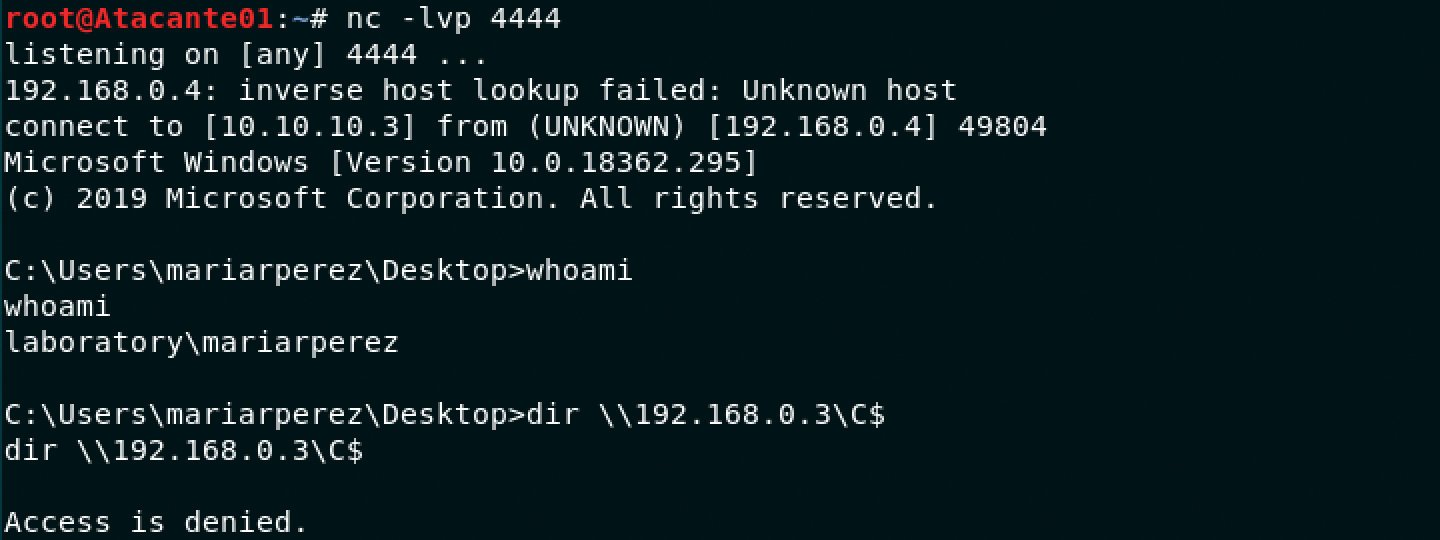
\includegraphics[width=15cm]{PTH/PTH1.png}
\end{center}
\caption{Reverse Shell interactiva sin privilegios.}
\label{PTH1}
\end{figure}

\item Si recogemos el tráfico intercambiado entre la máquina Cliente01 y el DC01, podemos ver que al intentar listar un directorio a través de la IP de éste se realiza a través del protocolo SMB utilizando el protocolo de autenticación NTLM donde el user es {\it LABORATORY\textbackslash{}mariarperez}. Al no tener privilegios, nos deniega el acceso (Figura \ref{PTH2}).
\begin{figure}[H] %[ht!] para here [b] para bottom [t] para top
\begin{center}
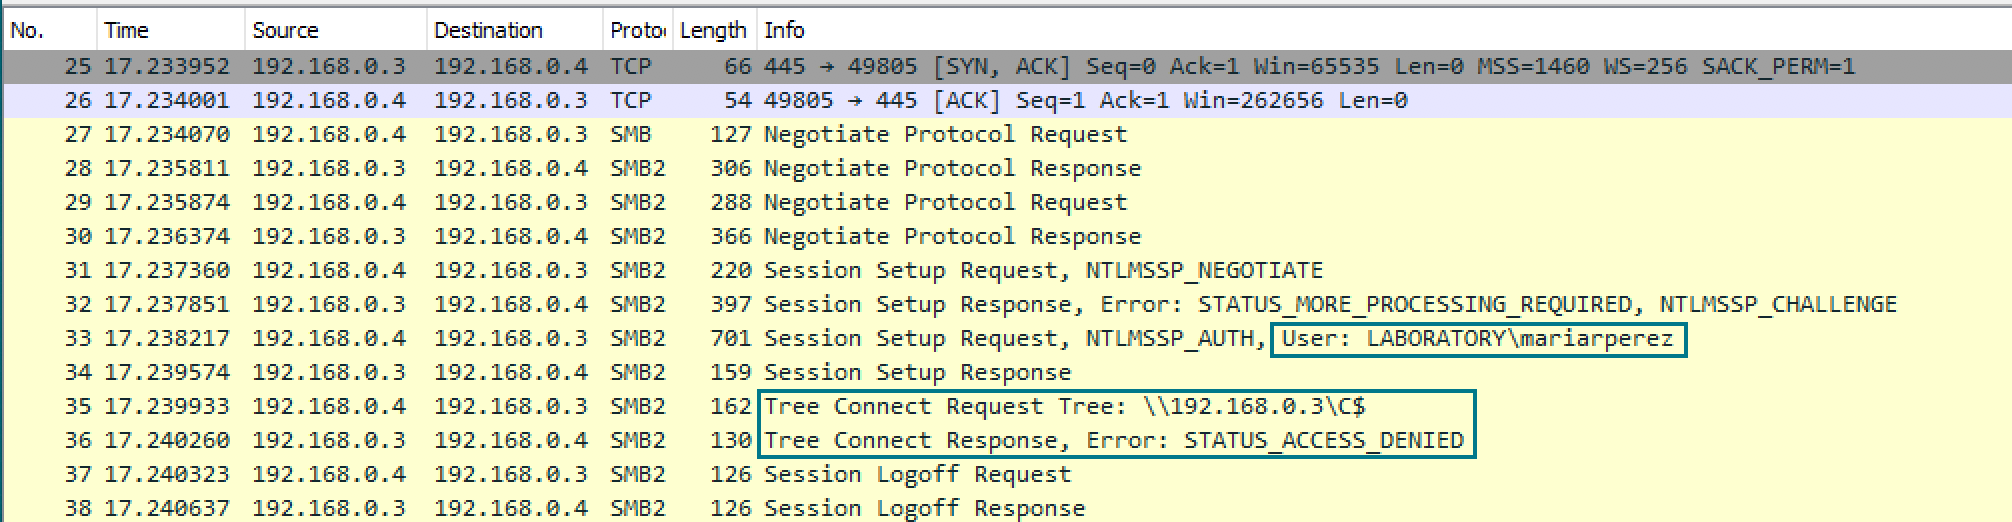
\includegraphics[width=15cm]{PTH/PTH2.png}
\end{center}
\caption{Paquetes intercambiados entre Cliente01 y DC01 - Sin pass the hash.}
\label{PTH2}
\end{figure}

\item  Al disponer de una sesión válida el usuario {\it federicogar} podemos obtener el hash de la contraseña del proceso LSASS. Para ello, se ha utilizado la herramienta Mimikatz~\cite{Capitulo5:Mimikatz} a través de los siguientes comandos (Figura \ref{PTH3}).
\begin{listing}[style=consola, numbers=none]
# privilege::debug
# sekurlsa::logonpasswords
\end{listing}

\begin{figure}[H] %[ht!] para here [b] para bottom [t] para top
\begin{center}
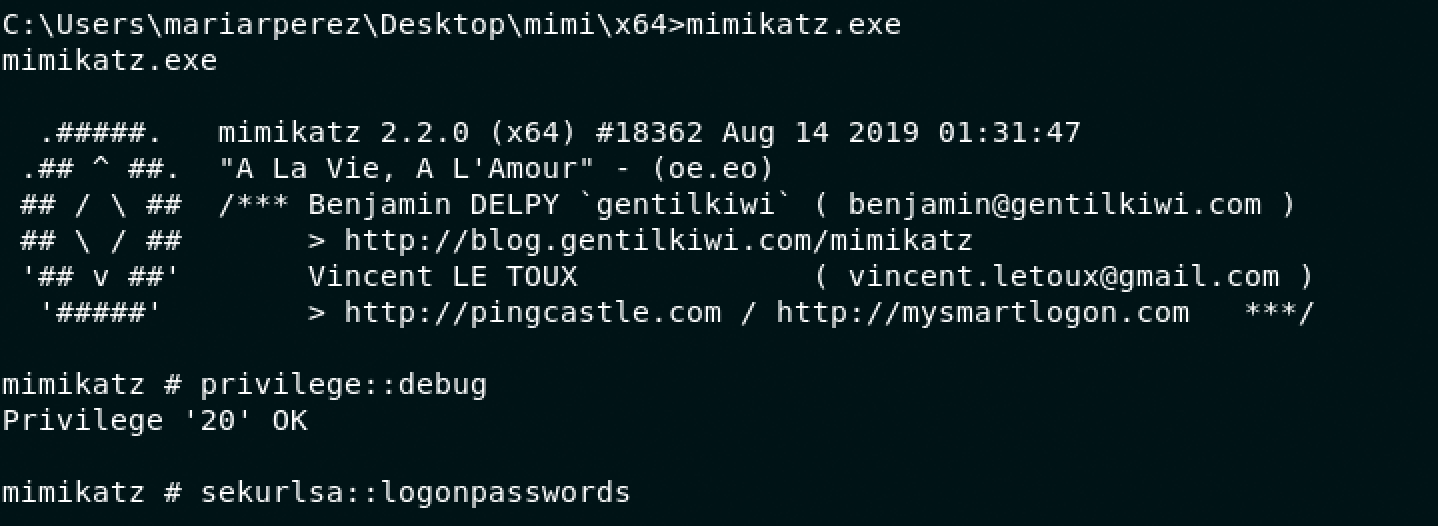
\includegraphics[width=15cm]{PTH/PTH3.png}
\end{center}
\caption{Comandos Mimikatz para listas sesiones activas.}
\label{PTH3}
\end{figure}

\item El comando anterior lista todos las sesiones activas en el usuario, por lo tanto, buscamos la que pertenece al usuario víctima y obtenmos el Hash NT (Figura \ref{PTH4}).
\begin{figure}[H] %[ht!] para here [b] para bottom [t] para top
\begin{center}
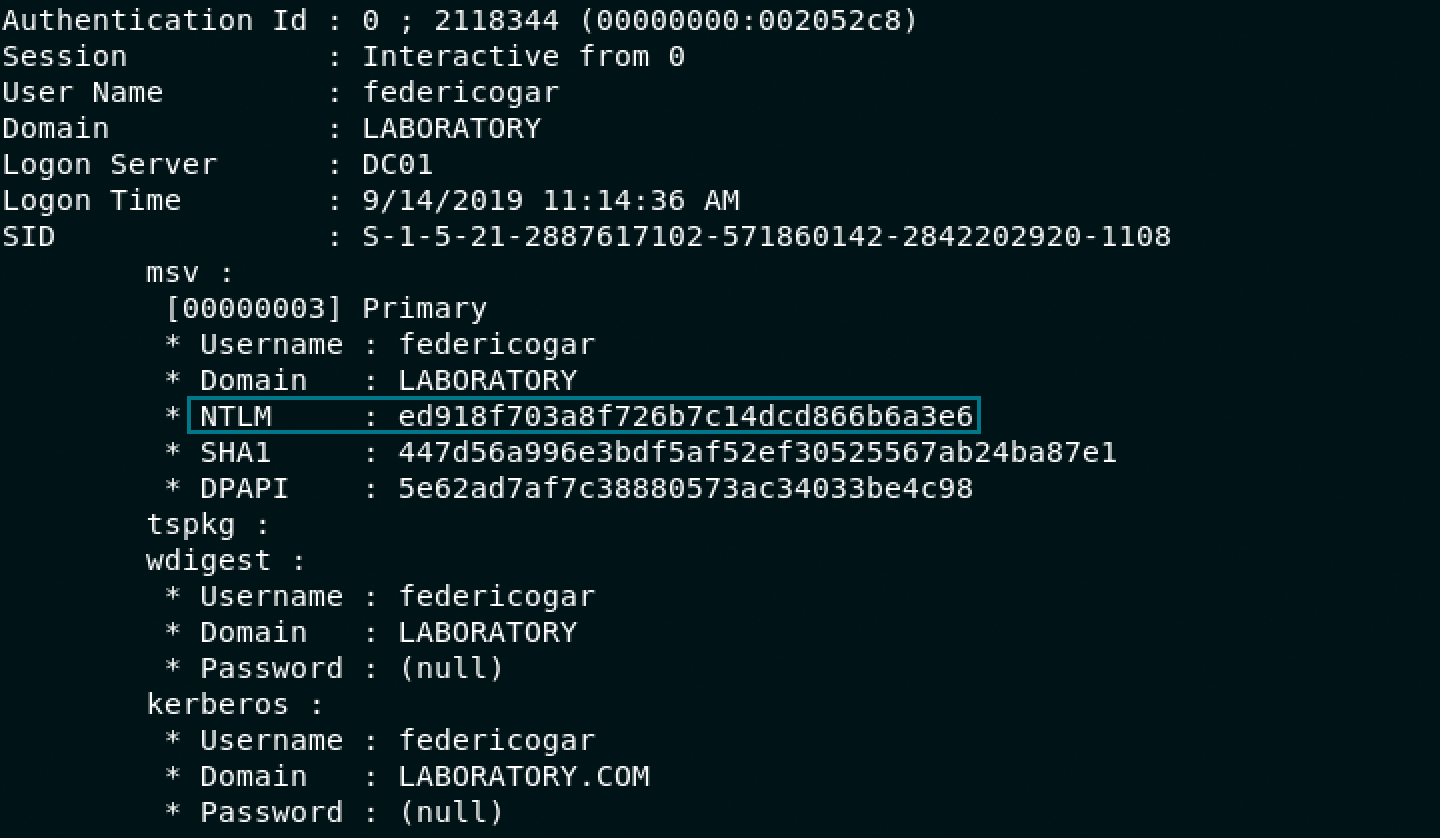
\includegraphics[width=15cm]{PTH/PTH4.png}
\end{center}
\caption{Hash del usuario víctima.}
\label{PTH4}
\end{figure}

\item La propia herramienta Mimikatz permite realizar el ataque Pass the Hash a través del siguiente comando, el resultado de este comando se puede observar en la Figura \ref{PTH5}.
\begin{listing}[style=consola, numbers=none]
# sekurlsa::pth /user:federicogar /ntlm:ed918f703a8f726b7c14dcd866b6a3e6 /domain:LABORATORY /run:cmd.exe
\end{listing}


\begin{figure}[H] %[ht!] para here [b] para bottom [t] para top
\begin{center}
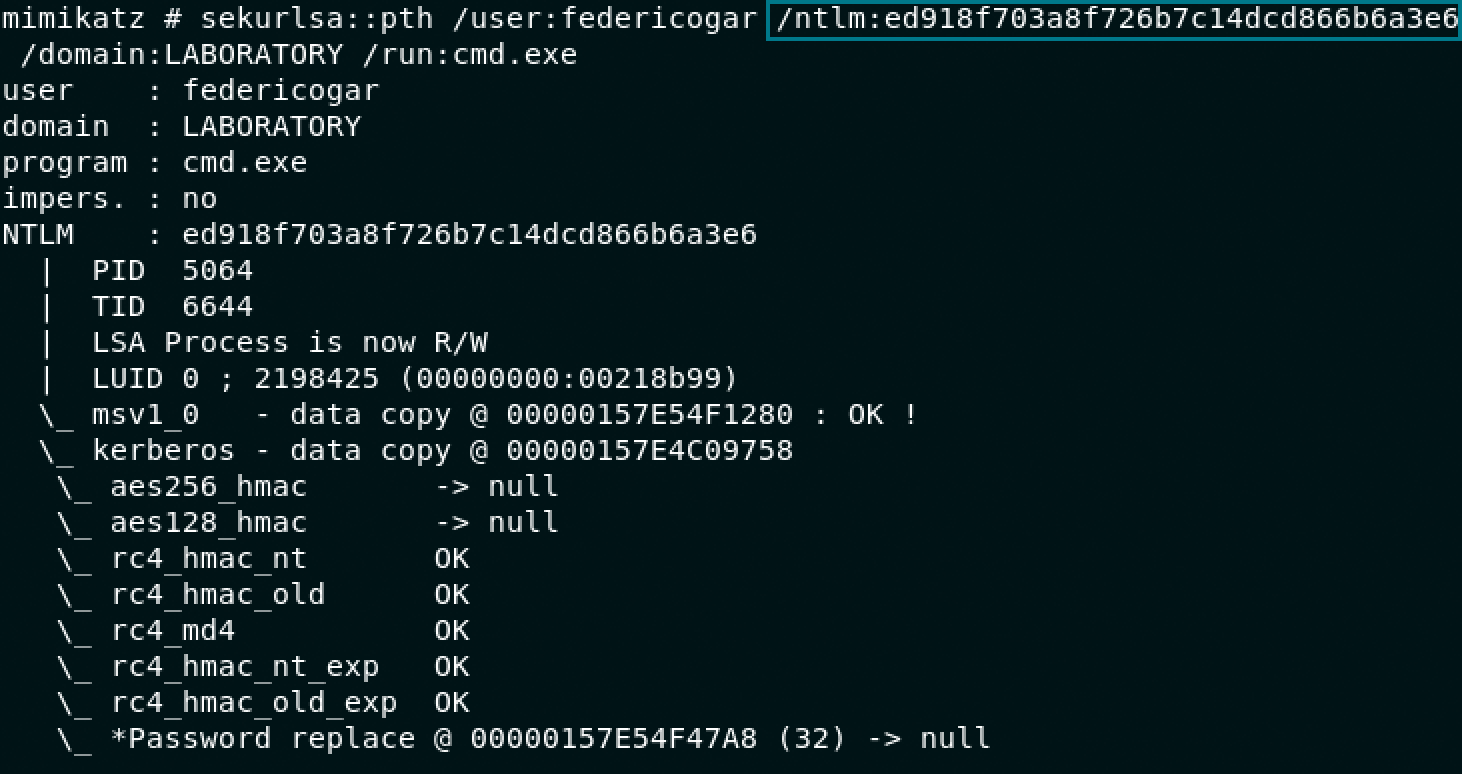
\includegraphics[width=15cm]{PTH/PTH5.png}
\end{center}
\caption{Pash the hash a través de la herramienta Mimikatz.}
\label{PTH5}
\end{figure}

\item En el comando anterior, se definió que ejecutar el comando {\it cmd.exe}, este comando se ejecutará en el Cliente01, por lo tanto, si queremos que se ejecute otra {\it Reverse Shell} con privilegios del uusario víctima sería necesario especificar otro comando. En la shell resultante (Figura \ref{PTH6}) podemos observar que aunque seguimos siendo el uusario {\it mariarperez} podemos listar los archivos de DC01. Esto es debido a que Mimikatz genera una nueva sesión para el usuario {\it mariarperez} y sobreescribe el contenido de las credenciales con el hash del otro usuario. 
\begin{figure}[H] %[ht!] para here [b] para bottom [t] para top
\begin{center}
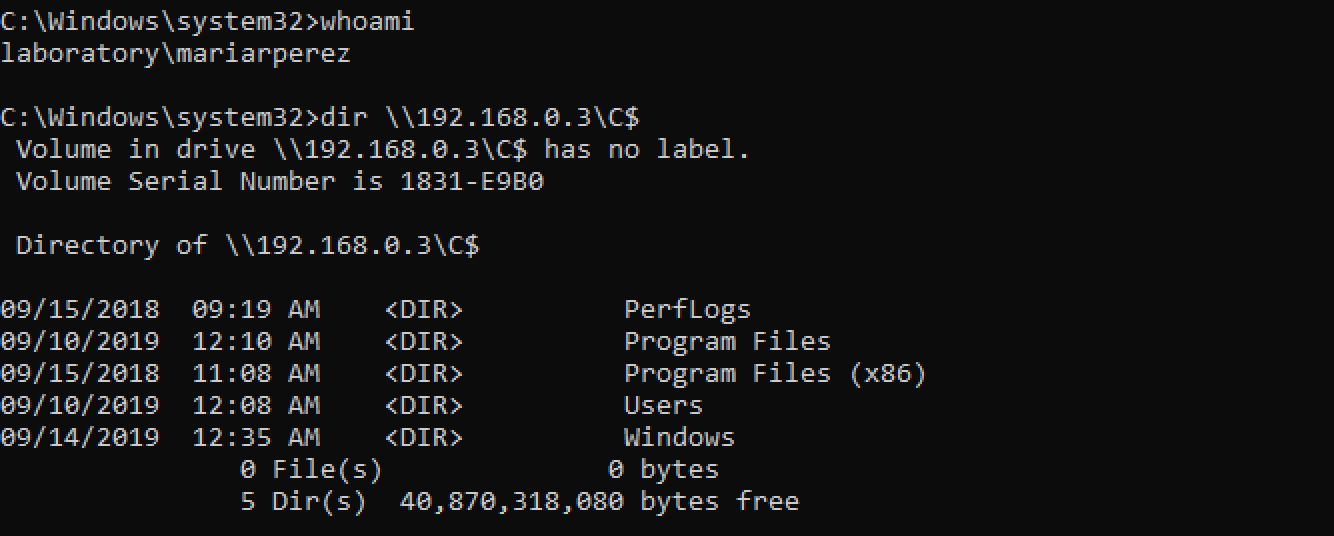
\includegraphics[width=15cm]{PTH/PTH6.png}
\end{center}
\caption{Ataque pass the hash realizado correctamente.}
\label{PTH6}
\end{figure}

\item Por último, al recoger el tráfico generado en esta comunicación podemos observar bastantes diferencias con la figura anterior, ahora el usuario es {\it federicogar} y se ha realizado el {\it Challenge-Response} de NTLM satisfactoriamente pudiendo listar los ficheros (Figura \ref{PTH7}).
\begin{figure}[H] %[ht!] para here [b] para bottom [t] para top
\begin{center}
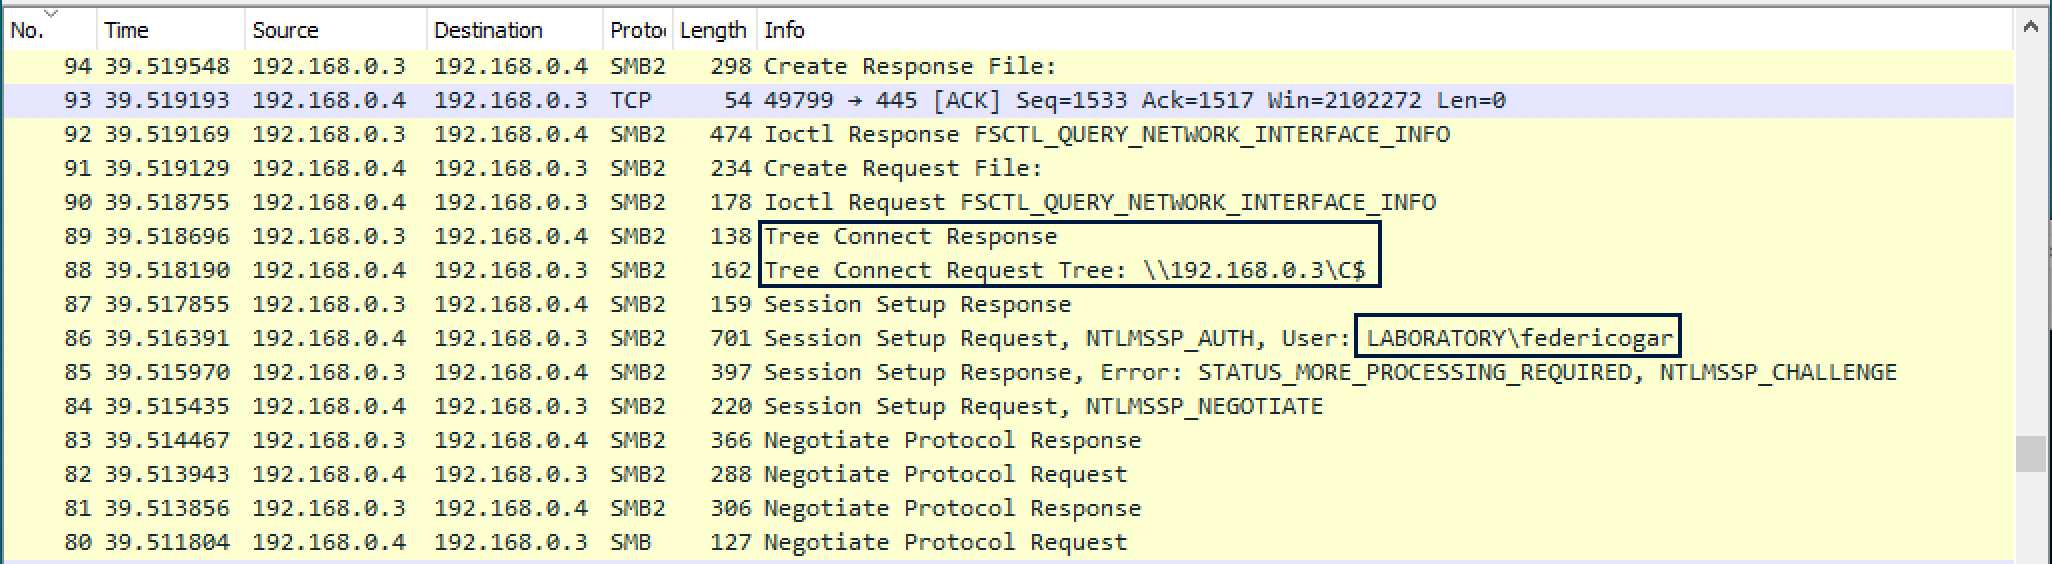
\includegraphics[width=15cm]{PTH/PTH7.png}
\end{center}
\caption{Paquetes intercambiados entre Cliente01 y DC01 - Con pass the hash.}
\label{PTH7}
\end{figure}

\end{enumerate}

\section{NTLM Relay}

\section{Overpass The Hash}

\section{Pass The Ticket}

\section{Golden/Silver Ticket}

\section{Kerberoast}
